\section{Front End}
The front end of the system deals with the input and output of the system, this will manipulate and process
the input into a form that can be used by the backend to perform the synthesis, seperating the front and backend
allows the i/o and the synthesis to be modified with no modification required for the other block,
for intance the output could be an BMP image or a surface within a gui, the details of the conversion are
irrelevent to the back-end, only that the data passed to it is in a format that is understood.

\subsection{Scene Input}
The scene input takes in a description of a scene that is to be rendered from a file, this scene description
will give a listing of each of the objects in the scene such as meshes, lights and camera. Each of these
objects are also described by a file that is listed in the scene file. Each of the scene files are text files
that are human readable, this allows the files to be easily modified. Each of these configuration files allows
for attributes to be reused such as a material describing a mirrored surface can be defined in a single material
file that can be referenced by multiple objects. below is a list of the different scene files that are defined
(details of each of the files can be found in the appendix).

\begin{description}
\item[.scene] Top level description of the scene
\item[.mesh] Description of a mesh, including material and surface data.
\item[.mat] Description of a objects surface properties.
\end{description}

\subsubsection{PLY mesh format}
One aspect of the mesh input file is a filename that referes to a PLY polygonal mesh, it was decided that using
a pre-existing file format for the input to system was benificial as it allowed for assets from 3D modeling
utilities to be used to create the test scenes as they contain the required functionallity to export to PLY
meshes. the choice of the PLY made because it is a human-readable format (a binary PLY format is available but
not supported by the system) and we specify this to be a key requirement of the system, 
using PLY also allowed for example meshed from the Stanford PLY reposotory which in turn provided a selection of
relitivly complex models that could be used during the production and testing.

\begin{figure}
\lstinputlisting[language=C]{../Code/data/scenes/cornell_box.scene}
\label{fig:scene_file_example}
\caption{Example Scene File}
\end{figure}

\subsection{Command Line Arguments}
The program that is created must be able to take in more than one scene file to be useful, by having command
line arguments this allows the scene file to be changed without recompiling the code, there are other options
that are available including the number of threads that will be used to perform the raytracing and the
resolution and name of the output file, this will allow for the system to be used in scripts, refer to
Appendix~\ref{chap:command-line-appendix} for full details of the command line options that are available.

\subsection{Image Output}
The image and gui block contains the code that will take the final pixel colours and present them to the screen
there will be two modes of operation, image output and GUI output, image output saves the image to a file such
as png or bmp.

\subsection{GUI}
In order to provide immediate feedback to the user it is nessaccarry to include a GUI in the system, this will
be a simple window that will display the progress of the system as it creates the images, this is usefull
for testing changes to a scene as it may be possible to see if the change has had the desired effect without
finishing what may be a costly render or to assure the user that a render is still running, the block level
design of the GUI can be found in Figure~\ref{fig:gui_design}.

\begin{figure}
\centering
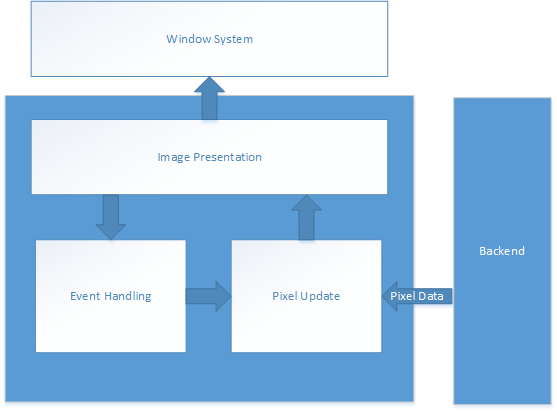
\includegraphics[width=0.7\textwidth]{./images/gui_design.png}
\caption{GUI design diagram}
\label{fig:gui_design}
\end{figure}

\subsection{Console Output and Logging}
In certain environments it is not possible to support a GUI (headless server) as a result the system includes
output on the console that inform the user of the progess of the render, this provides a visual disply of the
progress at each stage in the rendering and also any warnings that can be used to debug issues that arise
during the execution of the program.
